%%	PST4UserManual.tex
%	Thad Haines		
% 	Purpose:		Document to collect PST v4 changes/information that will end up being a pseudo user manual.
%	Notes:			Build with LuaLatex, use biber as bibliography backend.

\documentclass[12pt]{report}

%% Document Knowns
\newcommand{\CAPTitle}{Power System Toolbox 4 \\
	\vspace{2em}
	--User Manual--\\
	Documentation Version 0.0.0-b.2
}
\newcommand{\Author}{Thad Haines}
\newcommand{\Degree}{-}
\newcommand{\University}{-}
\newcommand{\Year}{2020}
\newcommand{\Subject}{Software Documentation}
\newcommand{\Keywords}{PST, Power System Toolbox, MATLAB, power system dynamics, AGC, variable time step integraion}

%%	pretty_preamble.tex
%	Thad Haines		Template
% 	Purpose:		Provide alternative to ugly thesis format.
%	Notes:			Included by thesis main.
%					Build with LuaLatex, use biber as bibliography backend.
%					Bibliography style can be changed below. see ***

%	Alteration History:		10/05/19	Added numbering to paragraphs to mimic subsubsubsections
%							10/11/19	Addition of lscape / pdflscape for landscape possibilities
%							10/17/19	Addition of minted package for purty code~
%							11/21/19	Use of glossaries package implemented.
%							11/30/19	Added siunitx for table formatting


% Tech specific formatting
\usepackage{setspace}
\setlength{\parindent}{0.5in}
\usepackage{indentfirst}
\usepackage{geometry}
\geometry{letterpaper, margin=1in}

%\usepackage{lscape} % for landscape pages
\usepackage{pdflscape} % for landscape pages - rotates digital page so text appears 'normal'

\usepackage{mathrsfs} % for laplace L

\usepackage{comment}
\usepackage{adjustbox}

\usepackage{enumitem} % for alteration of enumerate display 09/21/20

% Glossaries package configuration
\usepackage[nogroupskip, nonumberlist, nopostdot]{glossaries}
\setglossarystyle{long3colheader}
\renewcommand*{\entryname}{Term}
\renewcommand*{\descriptionname}{Definition}
\renewcommand*{\pagelistname}{} % remove page number col
\setlength{\glsdescwidth}{5 in} % width of description - may have to alter
\makeglossaries

% pretty commands for dual build
\newcommand{\fmAddAs}{chapter} % what to add aditional toc as (ugly = parts, pretty = chap)
\newcommand{\MTten}{\footnotesize}
\newcommand{\coverSkip}{2em}
\newcommand{\tocAbstract}{Abstract}
\newcommand{\tocDedication}{Dedication}
\newcommand{\tocAckno}{Acknowledgments}
\newcommand{\tocGlossary}{Glossary of Terms}

%*** Bibliography stuff
\usepackage[backend=biber,style=ieee, % bibliography style may be changed
sorting=nyt, % sorts by author, year, title
autocite=inline, sortcites=true, labelnumber=true, % for compressed cites
dashed=false, % show repeated authors (i.e. don't blank out names)
]{biblatex}
\addbibresource{bibliography.bib}
\nocite{*} % include non referenced citations

% for Altering Section titles to desired compact format.
\usepackage{titlesec} 
\titleformat{\chapter}
{\normalfont\LARGE\bfseries}{\LARGE \thechapter}{20pt}{\LARGE} 

\titlespacing*{\chapter}{0pt}{-30pt}{.25em}
\titlespacing{\section}{0pt}{0pt}{0pt}
\titlespacing{\subsection}{0pt}{0pt}{0pt}
\titlespacing{\subsubsection}{0pt}{0pt}{0pt}
\titlespacing{\bibliography}{0pt}{0pt}{0pt}

% Packages for filler text
\usepackage{blindtext} % for \blindtext -> Loerm ipsum dolor...
\usepackage{lipsum} % for short lines

% for maths and maths symbols
\usepackage{amsmath} 
\usepackage{amssymb}
\usepackage{commath}
\newcommand\numberthis{\addtocounter{equation}{1}\tag{\theequation}} % for simple \numberthis command to add equations to ...

% For list of equations - much pushing around to match other toc,lof...
% Required since list of equations not standard in report format
\usepackage[titles]{tocloft}
\newcommand{\listequationsname}{List of Equations}
\newlistof{thesisequations}{loe}{\listequationsname}
\newcommand{\eqcaption}[1]{
	\addcontentsline{loe}{thesisequations}{%\hspace{1.12em}  
	 \protect\numberline{\theequation} \hspace{1.85em} #1}\par\vspace{-2.5em}}%

%removal of 'chapter change' additional space in lot, lof
\usepackage{xpatch}
\makeatletter
\xpatchcmd{\@chapter}{%
	\addtocontents{lof}{\protect\addvspace{10\p@}}%
	\addtocontents{lot}{\protect\addvspace{10\p@}}%
}{}{}{}
\makeatother

%%% Add Figure zz: to list of figures 
\setlength{\cftfigindent}{0pt}  % remove indentation from figures in lof
\renewcommand{\cftfigaftersnum}{\quad}
\renewcommand{\cftfignumwidth}{4em}

%%% Add Table XX: to list of tables
\renewcommand{\cfttabaftersnum}{\quad}
\setlength{\cfttabindent}{0pt}  % remove indentation from tables in lot
\renewcommand{\cfttabnumwidth}{4em}

% for chapter leader dots
\renewcommand{\cftchapleader}{\cftdotfill{\cftdotsep}}

% For figure usage and linking
\usepackage{graphicx}
\graphicspath{ {figures/} }

% Caption formating footnotesize ~ 10 pt in a 12 pt document
\usepackage[font={footnotesize, bf}]{caption}

% For table formatting
\usepackage{booktabs}
\renewcommand{\arraystretch}{1.2}
\usepackage{floatrow}
\floatsetup[table]{capposition=top} % put table captions on top of tables

% for code listings with color 10/17/19
\usepackage{minted}
\usepackage{xcolor}

% for labeled listings 09/18/20
\usepackage{listings}
\renewcommand\lstlistlistingname{List of Listings} % rename page header
\lstset{basicstyle=\singlespacing,} % basic format of listing...
\makeatletter
\renewcommand*{\l@lstlisting}{\@dottedtocline{1}{0em}{2.3em}} % removing indent from main list of listings
\makeatother

% For header and footer control:
\usepackage{fancyhdr}
\pagestyle{fancy}
\fancyhf{}
\renewcommand{\headrulewidth}{0pt}
\rhead{\thepage}

% Redefine the plain page style so plain pages are same as fancy
\fancypagestyle{plain}{%
	\fancyhf{}%
	\rhead{\thepage}%
	\renewcommand{\headrulewidth}{0pt}% Line at the header invisible
	\renewcommand{\footrulewidth}{0pt}% Line at the footer nonvisible
}

% configurations of counters
\usepackage{chngcntr}
\setcounter{tocdepth}{5} % required to show subsubsections in toc
\setcounter{secnumdepth}{5} % required for x.x.x.x sections % Changed from 3 - 10/5/19

%%% Added for paragraph numbering to be subsubsection
\makeatletter
\renewcommand\paragraph{\@startsection{paragraph}{5}{\z@}%
            {-2.5ex\@plus -1ex \@minus -.25ex}%
            {1.25ex \@plus .25ex}%
            {\normalfont\normalsize\bfseries}}
\makeatother

% Command to correctly add page numbers to toc, lof, lot, loe...
\newcommand{\correctpagenumtoc}[1]{%
	\cleardoublepage
	\phantomsection
	\addcontentsline{toc}{\fmAddAs}{#1}}

% Fix header height
\setlength{\headheight}{15pt}

%%% SI unit x added for tables...
\usepackage[per-mode=fraction]{siunitx} % for si units and num
\sisetup{group-separator = {,}, group-minimum-digits = 3}

\usepackage{array} 		% for >{} column characterisctis
\newcolumntype{L}[1]{>{\raggedright\let\newline\\\arraybackslash\hspace{0pt}}m{#1}}
\newcolumntype{C}[1]{>{\centering\let\newline\\\arraybackslash\hspace{0pt}}m{#1}}
\newcolumntype{R}[1]{>{\raggedleft\let\newline\\\arraybackslash\hspace{0pt}}m{#1}}

% Silence warning that is known to not be a 'thing' when using ieee bibliography
% https://tex.stackexchange.com/questions/451192/file-english-ieee-lbx-not-found-ignoring-mapping-english-english-ieee
\usepackage{silence}
\WarningFilter{biblatex}{File 'english-ieee.lbx'}

% Packages enables content to function as links and describe default pdf behavior
\usepackage[hidelinks]{hyperref}
\hypersetup{
	pdftitle={\CAPTitle},
	pdfauthor={\Author},
	pdfsubject={\Subject},
	pdfkeywords={\Keywords},
	bookmarksnumbered=true,     
	bookmarksopen=true,         
	bookmarksopenlevel=3,       
	colorlinks=false,            
	pdfstartview=Fit,           
	pdfpagemode=UseOutlines,   
	pdfpagelayout=OneColumn
}
%% Flow chart specific packages
\usepackage{tikz}
%\usepackage{amsmath}
%\usepackage{comment}
\usetikzlibrary{shapes.geometric, arrows, positioning}
\usetikzlibrary{calc,shapes,shapes.multipart}
\tikzstyle{arrow} = [thick,->,>=stealth]

%% Flow chart custom shapes
% Terminal
\tikzstyle{terminal} = [rectangle, rounded corners, minimum width=5cm, minimum height=1cm,text centered, text width=4.5cm, draw=black]

% Process
\tikzstyle{process} = [rectangle, minimum width=5cm, minimum height=1cm, text centered,text width=4.5cm, draw=black]

% Decision
\tikzstyle{decision} = [diamond, aspect=1.8, minimum width=2cm, minimum height=1cm, text centered, text width=2cm, draw=black]

% Subprocess
\newcommand\ppbb{path picture bounding box}
\tikzset{
	subprocess/.style = {rectangle, draw=black, 
		minimum width=5cm, minimum height=1cm, inner xsep=3mm,
		text width =\pgfkeysvalueof{/pgf/minimum width}-2*\pgfkeysvalueof{/pgf/inner xsep},
		align=flush center,
		path picture={\draw 
			([xshift =2mm] \ppbb.north west) -- ([xshift= 2mm] \ppbb.south west)
			([xshift=-2mm] \ppbb.north east) -- ([xshift=-2mm] \ppbb.south east);
		},% end of path picture
	}
}

% bubble note
\tikzstyle{note} = [fill, ellipse,fill=gray!20, node distance=4cm, minimum height=1em, text width=3cm, text centered]

%Off page connector
\tikzset{
pageconD/.style={shape=signal,draw, signal to=south,minimum width=3em,text height=1.5em,align=center}
}
\tikzset{
pageconU/.style={shape=signal,draw, signal to=north,minimum width=3em,text height=1.5em,align=center}
}

%% For including only certain parts of document in build, uncomment :
%\includeonly{frontmatter/glossary} % Optional build modes
\nocite{} 
\newcommand{\tempPB}{\pagebreak \clearpage}
\newcommand{\uglyVspace}{\vspace{-0.75 em}} % used for creating spaces in front matter
\newcommand{\uglyPB}{ }  % used for creating spaces in front matter
\newcommand{\prettyPB}{\pagebreak \clearpage}
\begin{document}
\Large % for cover font size
\begin{titlepage}
	\pagenumbering{roman}
	\setcounter{page}{1}
	\onehalfspacing
	\topskip0pt
	\vspace{4em}
	\vspace*{\fill}
    \begin{center}
        \textbf{\CAPTitle}\\
        \vspace{2em}
        Last Document Build: \today
		\vspace{4em}
		\ \\ % removed by
        \Author \\  
      	\vspace{2em}
		%Last Update: \today
        %A thesis submitted in partial fulfillment of the\\ 
        %requirements for the degree of\\
	%	\vspace{2em}
        %\Degree\\
     %   \vspace{2em}
    %    \vspace{4em}
        %\University\\
        %\Year\\
       % \vspace{.5em}
       % \includegraphics[width=1.25in]{shield.png}
    \end{center}
	\vspace*{\fill}
\end{titlepage}

% Begin roman numbers after cover
\pagestyle{fancy}
\pagenumbering{roman}
\setcounter{page}{2}
\fancyfoot{} % clear footer
\fancyhead[R]{\thepage}

\normalsize
\setlength\parindent{0cm}
\onehalfspacing % for nicer look

%% Front matter
\vspace{2em} % for tech wonkyness
\chapter*{Power System Toolbox Introduction}
\addcontentsline{toc}{\fmAddAs}{Power System Toolbox Introduction}

% Note the required use of \vspace{1em} to seperate paragraphs.

Power System Toolbox (PST) is MATLAB code used to: 1) solve power flow problems; 2) simulate power-system transients; and 3) to linearize a power system model.  
All code is open-access and free.  
PST is widely used by researchers studying problems related to power-system dynamics.  
Its open access format enables researchers to customize models and operations to meet their unique needs.  
Being MATLAB based code, one can incorporate powerful MATLAB functions into their problem solving process.

\vspace{1em}
PST was the brain child of Dr. Joe Chow of Rensselaer Polytechnic Institute with the original version written by him and Dr. Kwok W. Cheung in the early 1990s.  
The late Mr. Graham Rogers made significant contributions and included it in his book \cite{rogers1999}.  
Many others have added customized models and variations over the past two plus decades. 

\vspace{1em}
The basis for the version of PST presented in this document is version 3, available from Dr. Chow’s webpage (\href{https://www.ecse.rpi.edu/~chowj/}{https://www.ecse.rpi.edu/~chowj/}) with added customizable current-injection functions written by Dr. Dan Trudnowski from Montana Technological University. 
\vspace{2em} % for tech wonkyness
\chapter*{User Manual Introduction}
\addcontentsline{toc}{\fmAddAs}{User Manual Introduction} %%% ugly = ALL CAPS
%\addcontentsline{toc}{\fmAddAs}{\tocAbstract}%%% All caps == ugly
% Note the required use of \vspace{1em} to seperate paragraphs.

%A brief explanation of the user manual purpose and major content would make sense.
The purpose of this user manual is to document work done on PST 3 to form PST 4. 
It is meant only to augment the previous user manuals and other available documentation about \mbox{PST} \cite{chow1992, PST2LFTut, PST3manual, chow2015}.
%
Major code changes presented include 
how global variables are handled
and the
functionalization of the non-linear simulation routine.

\vspace{1em}
Descriptions of new models created for
inverter based resources
%power (or current) injection, 
%a voltage source behind a reactance,
and
automatic generation control
are also presented.
Additionally, work to add functionality to PST such as
variable time step integration routines,
generator tripping, % mention un-tripping
and
code compatibility with Octave
is documented.



\vspace{1em}
To demonstrate and debug new and old PST capabilities, an example library has been created and brief explanations of select examples is be included in this document.
Unfortunately, due to time constraints, details may be rather lacking.
however,  the code examples have been checked for functionality and should work as designed.

%and intentions may only matter so much.

\vspace{1em}
Finally, it is worth noting that all source code, examples, and other research documentation can be accessed at 
\href{https://github.com/thadhaines/MT-Tech-SETO/tree/master/PST}{https://github.com/thadhaines/MT-Tech-SETO/tree/master/PST}. 
% inclusions from template, may not be required.
%\chapter*{Dedication}
\addcontentsline{toc}{\fmAddAs}{\tocDedication}%%% all caps == ugly
\setlength\parindent{0cm}

For you... 
\\And others too.
\chapter*{Acknowledgments - WIP}
\addcontentsline{toc}{\fmAddAs}{\tocAckno} %%% ugly = ALL CAPS

More officially worded:
\begin{itemize}
\itemsep 0 em
\item Original Creators
\item Known major contributors
\item funding that made \emph{this} work possible.
\end{itemize}


%% Table of contents, lists of tables,figures, equations
% \correctpagenumtoc enables content line to be defined before table or list command is executed
\renewcommand{\contentsname}{Table of Contents \vspace{-.5em}}
\correctpagenumtoc{Table of Contents} 
\tableofcontents

\correctpagenumtoc{List of Tables}
\listoftables

\correctpagenumtoc{List of Figures}
\listoffigures

\correctpagenumtoc{List of Equations}
\listofthesisequations

\correctpagenumtoc{List of Listings} % added 09/18/20 - works, use for code listings
\lstlistoflistings


\onehalfspacing
\chapter*{Glossary of Terms}
\addcontentsline{toc}{\fmAddAs}{\tocGlossary} %%%%
\vspace{-2em}
% There are may be a better way to do this (i.e. use of glossaries package)
% Obviously, A table is used for now.

% using the glossaries package requires the installation of perl.
% additionally, the glossaries package reuires a seperate build of the glossary so that t prints at all (similar to the bibliography using biber)
\renewcommand*{\glsclearpage}{} % remove pagebreak pre-glossary
\renewcommand{\glossarysection}[2][]{} % remove auto glossary title

\newglossaryentry{ACE}{name={ACE}, description={Area Control Error }}
\newglossaryentry{AC}{name={AC}, description={Alternating Current}}
\newglossaryentry{DC}{name={DC}, description={Direct Current}}
\newglossaryentry{PU}{name={PU}, description={Per-Unit}}
\newglossaryentry{SACE}{name={SACE}, description={Smoothed ACE}}
\newglossaryentry{PI}{name={PI}, description={Proportional and Integral}}
\newglossaryentry{PST}{name={PST}, description={Power System Toolbox}}
\newglossaryentry{RACE}{name={RACE}, description={Reported ACE}}
\newglossaryentry{DACE}{name={DACE}, description={Distributed ACE}}
\newglossaryentry{PSS}{name={PSS}, description={Power System Stabilizer }}
\newglossaryentry{AGC}{name={AGC}, description={Automatic Generation Control }}
\newglossaryentry{WECC}{name={WECC}, description={Western Electricity Coordinating Council }}
\newglossaryentry{NERC}{name={NERC}, description={North American Electric Reliability Corporation }}
\newglossaryentry{FERC }{name={FERC}, description={Federal Energy Regulatory Commission }}
\newglossaryentry{EIA}{name={EIA}, description={ United States Energy Information Administration}}
%\newglossaryentry{CTS}{name={CTS}, description={ Classical Transient Stability}}
\newglossaryentry{ODE}{name={ODE}, description={ Ordinary Differential Equation }}
%\newglossaryentry{US}{name={US}, description={United States of America }}
%\newglossaryentry{RTO}{name={RTO}, description={Regional Transmission Organization}}
%\newglossaryentry{ISO}{name={ISO}, description={Independent Service Operator}}
%\newglossaryentry{SI}{name={SI}, description={International System of Units}}
\newglossaryentry{Hz}{name={Hz}, description={Hertz, cycles per second}}
\newglossaryentry{W}{name={W}, description={Watt, Joules per second}}
\newglossaryentry{J}{name={J}, description={Joule, Neton meters, Watt seconds}}
%\newglossaryentry{BES}{name={BES}, description={Bulk Electrical System}}
%\newglossaryentry{BA}{name={BA}, description={Balancing Authority}}
\newglossaryentry{P}{name={P}, description={Real Power}}
\newglossaryentry{Q}{name={Q}, description={Reactive power}}
\newglossaryentry{VAR}{name={VAR}, description={Volt Amps Reactive}}
%\newglossaryentry{IC}{name={IC}, description={Interchange}}
\newglossaryentry{VTS}{name={VTS}, description={Variable Time Step}}
\newglossaryentry{FTS}{name={FTS}, description={Fixed Time Step}}

\glsaddall % so that there is no need to call \gls{label} for each term
\printglossaries


\begin{comment}
% table style glossary for record...

\begin{table}[h]
	\begin{tabular}{@{} p{.25\linewidth} p{.7\linewidth} @{}} %\toprule 
	\textbf{Term} & \textbf{Definition}\\
	%	
	\LaTeX 			& A document preparation system. Favors logical design over visual design. Reportedly widely used in academia... \\
	PSLF 	&	Positive Sequence Load Flow. GE's power system simulation software.\\
	PSDS	&	PSLF Dynamic subsystem.\\
	PSS		&	Power System Stabilizer \\
	AGC		&	Automatic Generation Control \\
	LFC		&	Load Frequency Control \\
	WECC	&	Western Electricity Coordinating Council \\
	NERC	&	North American Electric Reliability Corporation \\
	FERC 	&	Federal Energy Regulatory Commission \\
	PSLTDSim &	Power System Long-Term Dynamic Simulator\\
	LTD		& 	Long-Term Dynamic. May also refer the type of simulation performed by PSLTDSim.\\

	\end{tabular}
\end{table}

\end{comment}


% Body Format
\setlength\parindent{0.5in}
\doublespacing
\pagenumbering{arabic}
\setcounter{page}{1} % Arabic Numbers start at the begining of chapter 1
\setcounter{table}{0}

%% Body of document goes here
% file to contain information on the history of PST versions
%==============================================================================
\chapter{PST Version History}

%If it seems wise to include a history about previous PST versions, this file can be included.

% copied from versioning document 09/03/20, modified as deemed fit

\section*{Current Versions}
\begin{itemize}
\itemsep 0 em
\item 2.3 - Based on PST 2, includes Dan Trudnowski's pwrmod, ivmmod, and generator tripping modifications.
\item 3.0 - From Joe Chow's website. 
Includes fixes and alterations. 
Notably multiple DC lines and PSS modifications.
\item 3.1 - Based on 3.0, includes Dan Trudnowski's pwrmod and ivmmod models in non-linear simulation. 
pwrmod included linear simulation and various model patches. 
Multiple generator tripping code is included, but untested.
\item 3.1.1 - Based on 3.1. Ryan Elliott's version with energy storage and updated linear simulation along with various other fixes and code cleanup alterations. 
\item SETO - Based on 3.1. New global structure. 
Includes automatic generation (AGC) models and variable time step (VTS) options. 
Also includes many patches as documented in 
\href{https://github.com/thadhaines/MT-Tech-SETO/tree/master/researchDocs/TEX/one-offs/200709-PSTsetoVersionChanges}{PSTsetoVersionChanges}. 
% 
Will become 4.0 after clean up actions taken.
\item 4.0.0-aX - Alpha version of PST 4 based on SETO version. 
Includes a refined VTS routine, confirmed multi-generator tripping, and improved AGC action/modulation.
Examples in repository will be re-worked/updated and cleaned to use this version, 
documentation of changes will be updated, 
and PST code will be cleaned up where possible.
May go into beta, which may then go into the `release candidate' phase, but may also just turn into 4.0.0.
\end{itemize}

\section*{Possible Future Versions}
\begin{itemize}
\itemsep 0 em
\item 4.0.0 - Finished VTS, AGC, code cleanup, example library, and documentation work by Thad Haines.
\item 4.1.0 - Based on 4.0.x - planned to incorporate energy storage models for non-linear simulation and possibly the updated linear simulation based on 3.1.1. Examples of \verb|ess| model use required.
\end{itemize}
% file to contain information on the various model fixes from version 3
%==============================================================================
\chapter{General Model or Bug Fixes}

This content will likely be separated into the changes/additions section as not all following sections are specific to code fixes but also additions/changes.
%content copied from PSTsetoVersionChanges on 09/03/20 -thad 

The purpose of this section is to record changes of note made to PST over the course of the SETO work that may be worth not forgetting about.
It should be noted that PST SETO is based on PST version 3 and not \textbf{all} changes are recorded here.


%===========================================================================================================
\section{exc\_dc12}  
In 2015 there were `errors' corrected in the saturation block that create differences between version 2 and 3 of this model.
Effects are noticeable, but a solution hasn't been investigated yet.

%===========================================================================================================
\section{exc\_st3}  
Corrected theta index to \verb|n_bus| from \verb|n| per Ryan Elliott.
Corrected simple \verb|*| to \verb|.*| int the \verb|if ~isempty(nst3_sub)| section.

%===========================================================================================================
\section{mac\_tra}  
Commented out code that prevented the setting equal of the transient reactances.

%===========================================================================================================
\section{lmod and rlmod}  
Fixed state limiting.
 While if over-limit, the derivative was set to zero, the state was not set to the maximum/minimum value correctly.



% file to contain information on variable changes (globals) and new models and functionality 
% specicaly (IVMMOD PWRMOD AGC VTS machine tripping)
%==============================================================================
\chapter{Changes and Additions}
It's assumed the last version is 3.


Maybe make a note about Experimental features (VTS, un-tripping)

\begin{itemize}
\item License
\item IMVMOD
\item PWRMOD
\item Machine tripping
\item Global Variable Structure
\item \verb|s_simu| Functionalization / clean up
\item AGC
\subitem areas, average frequency
\item VTS
\subitem differences from FTS (Huen's)
\item Speed up
\item Zeroing derivatives
\item Octave Compatibility
\end{itemize}
% file to contain information on general operation of v4
% s_simu, flochart, linear sim....
%==============================================================================
\chapter{PST Operation Overview}

This is likely to include a flow chart/ multiple flow charts.

Mention partitioned explicit method via Huen's, partitioned implicit via VTS.

Overview of running \verb|s_simu| in batch or stand alone mode.

copying of modulation files

%==============================================================================
\section{Simulation Loop}
The complete simulation loop code is shown below.
This code was copied from \verb|s_simu_BatchVTS| with corresponding line numbers.

\begin{minted}[
		frame=lines,
		framesep=2mm,
		baselinestretch=1.2,
		bgcolor=gray!13,
		fontsize=\footnotesize,
		linenos,
		firstnumber=362,
		breaklines
				]{MATLAB}
%% Simulation loop start
warning('*** Simulation Loop Start')
for simTblock = 1:size(g.vts.t_block)
    
    g.vts.t_blockN = simTblock;
    g.k.ks = simTblock; % required for huen's solution method.
    
    if ~isempty(g.vts.solver_con)
        odeName = g.vts.solver_con{g.vts.t_blockN};
    else
        odeName = 'huens'; % default PST solver
    end
    
    if strcmp( odeName, 'huens')
        % use standard PST huens method
        fprintf('*** Using Huen''s integration method for time block %d\n*** t=[%7.4f, %7.4f]\n', ...
            simTblock, g.vts.fts{simTblock}(1), g.vts.fts{simTblock}(end))
        
        % add fixed time vector to system time vector
        nSteps = length(g.vts.fts{simTblock});
        g.sys.t(g.vts.dataN:g.vts.dataN+nSteps-1) = g.vts.fts{simTblock};
        
        % account for pretictor last step time check
        g.sys.t(g.vts.dataN+nSteps) = g.sys.t(g.vts.dataN+nSteps-1)+ g.sys.sw_con(simTblock,7);
        
        for cur_Step = 1:nSteps
            k = g.vts.dataN;
            j = k+1;
            
            % display k and t at every first, last, and 50th step
            if ( mod(k,50)==0 ) || cur_Step == 1 || cur_Step == nSteps
                fprintf('*** k = %5d, \tt(k) = %7.4f\n',k,g.sys.t(k)) % DEBUG
            end
            
            %% Time step start
            initStep(k)
            
            %% Predictor Solution =========================================
            networkSolutionVTS(k, g.sys.t(k))
            monitorSolution(k);
            dynamicSolution(k)
            dcSolution(k)
            predictorIntegration(k, j, g.k.h_sol)   % g.k.h_sol updated i_simu
            
            %% Corrector Solution =========================================
            networkSolutionVTS(j, g.sys.t(j))
            dynamicSolution(j)
            dcSolution(j)
            correctorIntegration(k, j, g.k.h_sol)
            
            % most recent network solution based on completely calculated states is k
            monitorSolution(k);
            %% Live plot call
            if g.sys.livePlotFlag
                livePlot(k)
            end
            
            g.vts.dataN = j;                        % increment data counter
            g.vts.tot_iter = g.vts.tot_iter  + 2;   % increment total solution counter
            g.vts.slns(g.vts.dataN) = 2;            % track step solution
        end
        % Account for next time block using VTS
        handleStDx(j, [], 3) % update g.vts.stVec to initial conditions of states
        handleStDx(k, [], 1) % update g.vts.dxVec to initial conditions of derivatives 
        
    else % use given variable method
        fprintf('*** Using %s integration method for time block %d\n*** t=[%7.4f, %7.4f]\n', ...
            odeName, simTblock, g.vts.t_block(simTblock, 1), g.vts.t_block(simTblock, 2))
        
        % feval used for ODE call - could be replaced with if statements.
        feval(odeName, inputFcn, g.vts.t_block(simTblock,:), g.vts.stVec , options);
        
        % Alternative example of using actual function name:
        %ode113(inputFcn, g.vts.t_block(simTblock,:), g.vts.stVec , options);
    end
    
end% end simulation loop
\end{minted}
% file to contain information on examples
%==============================================================================
\chapter{Examples Explained - WIP}
As github as many examples, this is a chapter to explain what the purpose of them is and detail non-linear vs linear operation of examples that do such things.

\begin{itemize}
\item Experimental VTS
\item AGC
\item AGC interchange modulation
\item Extended term with VTS
\item Hiskens NE model via Ryan
\item MiniWECC via Dan
\item Experimental Un-tripping
\item Modulation via \verb|_mod| files
\item Linear simulation where applicable
\end{itemize}

Variables to note in associated examples (where \verb|x| is the internal model number):
\begin{itemize}
\item exciter $V_{ref} = $ \verb|g.exc.exc_pot(x,3)|
\item governor $P_{ref} = $ \verb|g.tg.tg_pot(x,5)|
\item governor $\omega_{ref} = $ \verb|g.tg.tg_con(x,3)|
\end{itemize}

\pagebreak
\section{Automatic Generation Control (AGC)} 
A variety of examples were created for AGC testing.
While some may use VTS, this section covers information only related to AGC.
The VTS example section contains VTS specific information.

The \verb|0-examples/AGC| folder contains all system and modulation files associated with the AGC examples.
The \verb|run***| files are designed to run PST in using the batch mode.
\section{Variable Time Step - WIP}
% file to contain information on loose ends or things generaly unfinished
%==============================================================================
\chapter{Loose Ends - WIP}
As software development is never actually `done', this chapter is meant to contain any loose ends that felt relevant.
%The below is copied from the most recent weekly (09/02/20) and some minor additions

\begin{enumerate}
	\item As infinite buses don't seem to be used in dynamic simulation, they were not converted to use the golbal g.
	\item \verb|tgh| model was not converted for use with global g. (no examples of tgh gov)
	\item In original (and current) \verb|s_simu|, the global \verb|tap| value associated with HVDC is over-written with  a value used to compute line current multiple times. \\It probably shouldn't be.
	\item Constant Power or Current loads seem to require a portion of constant Impedance.
	\item PSS design functionality not explored.
	\item No examples of of delta P omega filter or user defined damping controls for SVC and TCSC models
	\item Differences in \verb|mac_ind| between PST 2 and 3 seem backward compatible, but this is untested.
	\item DC is not implemented in VTS. It seems like DC models should be combined into the main routine if so desired. Seems counter intuitive / (not very possible) to do multi-rate variable time step integration...
	\item AGC capacity should consider defined machine limits instead of assuming 1 PU max.
	\item AGC should allow for a `center of inertia' frequency option instead of the weighted average frequency.
	\item A method to initialize the power system with tripped generators should be devised and occur before the first power flow solution.
	\item A method to zero derivatives of any model attached to a tripped generator should be created to enable VTS to optimize time steps.
	\item Re-initializing a tripped generator in VTS will likely require indexing the \verb|g.vts.stVec|. This could be aided by adding indices to the \verb|g.vts.fsdn| cell.
	\item miniWECC DC lines (modeled as power injection) are not included in AGC calculations as the power does not travel over any simulated lines.
	\item If a machine has been tripped, the Y matrix is adjusted and reduced every time step. This repeated action could be made more efficient.
\end{enumerate}


% chapter01 and chapter02 are template docs to show how template works - they are not intended to be included in final document.
%\chapter{Basic Formatting}
This chapter will show basic formatting of text, figures, tables and equations. It will also be mostly filled with `dummy' text so there is something to look at.

\section{Body Text}
Body text has a $1/2$ inch indent on all paragraphs and double spaced lines.
\lipsum[6]
\section{Figures, In-Text Citations, and Footnotes}
Figure~\ref{fig:athletic logo} is an example of how images can be formatted. Additionally, citations to references will be shown such \cite{latexcompanion}. Footnotes\footnote{This is a footnote text message that doesn't offer much information.} will behave like this\footnote{This is another footnote.}.

\begin{figure}[!ht]
	\centering
	\footnotesize
	
\includegraphics[width=2in]{test/athletic-bw.png}
	\caption{An Athletic logo?}
	\label{fig:athletic logo}
\end{figure}\vspace{-1em} % can be useful to pull following text closer... sometimes, other times messes up format.

A larger graphic example is shown on Page~\pageref{fig:ramp test 1} as Figure~\ref{fig:ramp test 1}. \lipsum[8] 

\begin{figure}[!ht]
	\centering
	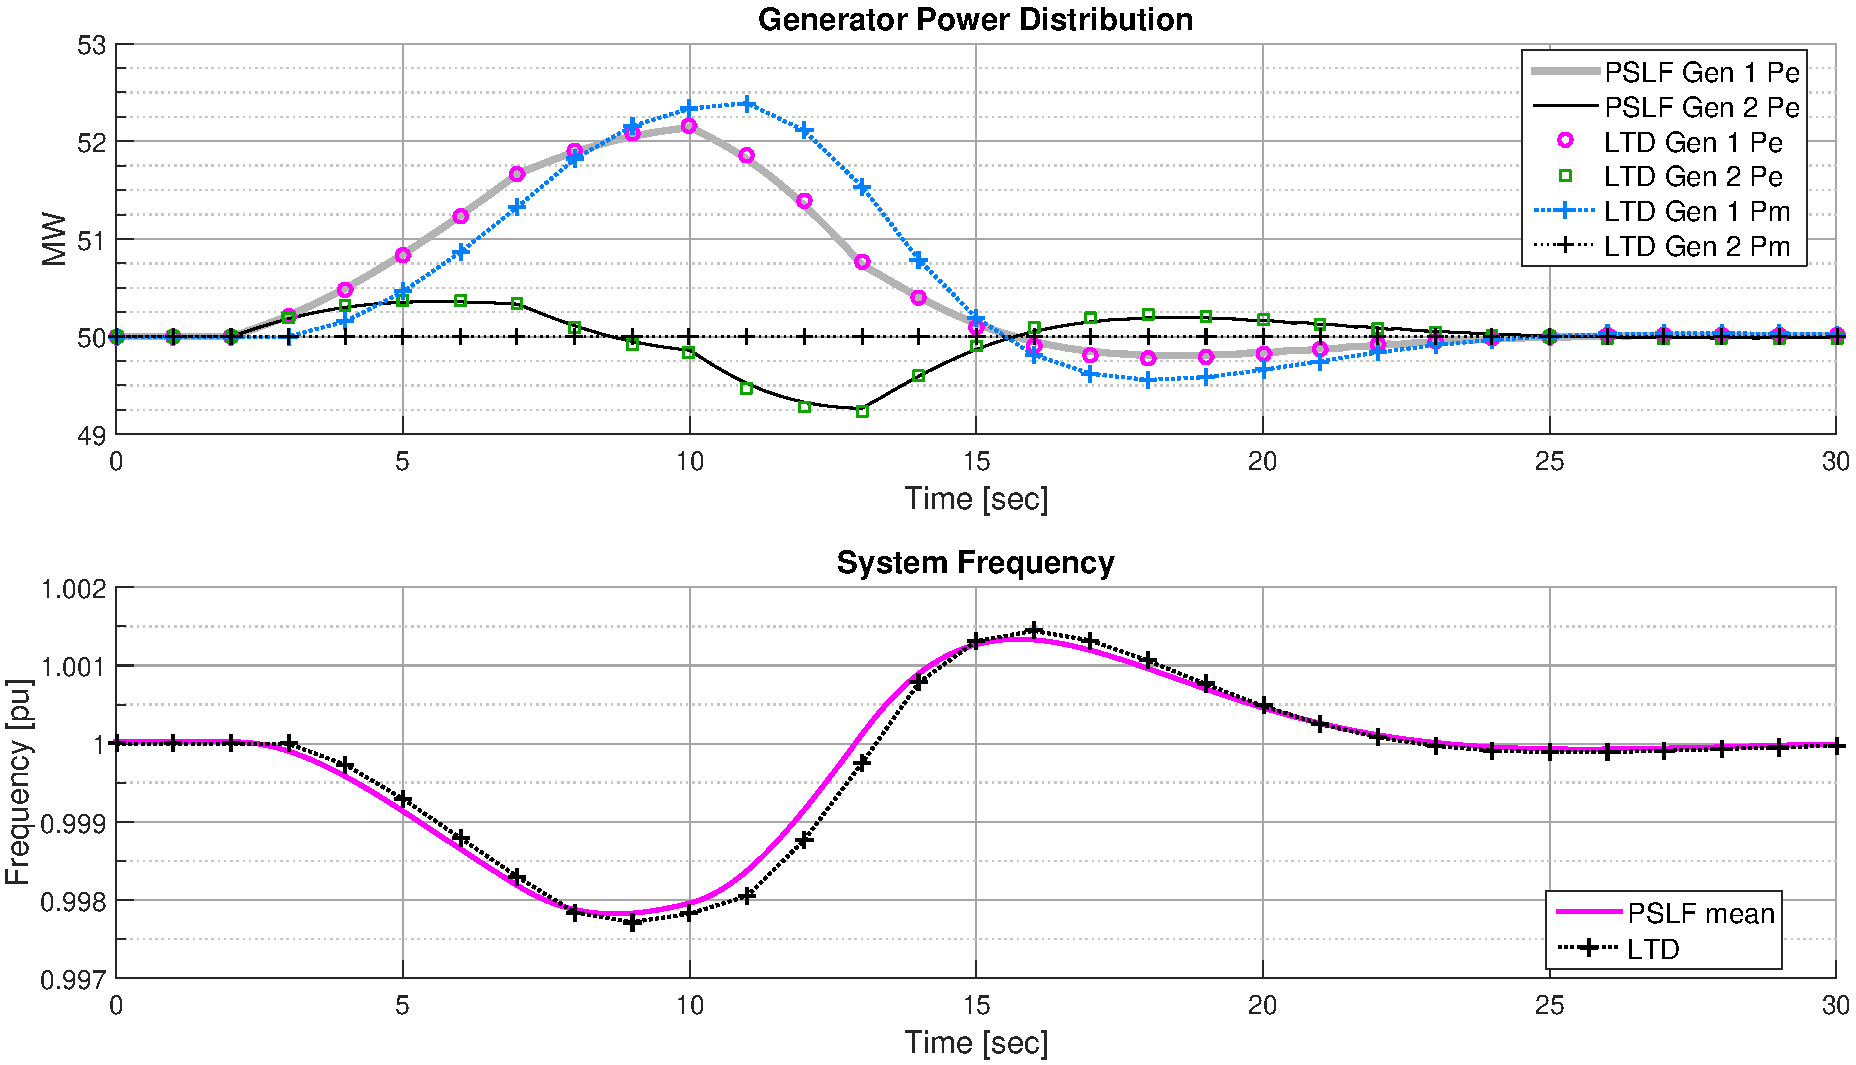
\includegraphics[width=\linewidth]{test/ramp1sec.pdf}
	\caption[60 Second Ramp Test.]{This is a fairly large graphic but can easily be set to any desired width. Additionally, this is a super long caption that would break the table of contents formatting if it weren't for an optional `short title' parameter. There's even a citation in here\cite{stajcar}.}
	\label{fig:ramp test 1}
\end{figure}%\vspace{-1em}

\lipsum[15]

\section{Equations}
	A somewhat fancy equation involving symbols and an integral is pretty easy to put together. \lipsum[5] %
	\begin{equation}{\label{eq:ssSoln}}
		x(t) = \Phi(t) x(0) + \int_{0}^{t}\Phi(t-\tau)Bu(\tau) \text{d}\tau.
	\end{equation}\eqcaption{An example of optional equation captions}

	\lipsum[6]\ Unlike Equation~\ref{eq:ssSoln}, Equation~\ref{eq:one} is pretty basic.%
	\begin{equation}{\label{eq:one}}
		a+b=c
	\end{equation}\eqcaption{.}
	
	Aligned rows of equations are also possible using the \verb|align*| environment and a custom \verb|numberthis| command. The following math is very math.
	\begin{align*}
		G(\$) &= \dfrac{20}{\$(\$+5)(\$+10)}\\
		\zeta = 0.59116 &, \Phi_M = 58.59\\
		\therefore \omega_{\Phi_M} &= \omega \angle -121.41^\circ\\
		\text{From Bode: } \omega_{\Phi_M} &= 1.9 \\
		\abs{\omega_{\Phi_M}} &= -14.3 \\
		\therefore K &= 10^\frac{14.3}{20} =5.188 \text{ abs} \numberthis \label{eq:align}
	\end{align*}\eqcaption{Some Gain Calculation}

\section{Tables}
Tables can look like Table~\ref{tab:exp1}. Notice the slimming effect of no vertical lines\ldots .
 Quisque vehicula, urna sed
ultricies auctor, pede lorem egestas dui, et convallis elit erat sed nulla. Donec luctus. 

\begin{table}[h]
	\centering
	\begin{tabular}{@{} l r r r r @{}} 	
		\toprule % @ signs to remove extra L R space
		\footnotesize % this will make the table font 10pt
		& \multicolumn{1}{c}{Experiment 1}	& \multicolumn{1}{c}{Experiment 2}	& \multicolumn{1}{c}{Experiment 3}	& \multicolumn{1}{c}{Experiment 4} \\
		\midrule
		Old	& 29.631	& 17.333	& 222.999	& 11.222 \\
		Not Old	& 54.321	& 166.233	& 556.123	& 54.666 \\
		Almost New	& 118.791 &	54.289 &	445.321 &	88.122 \\
		New& 	222.897	& 10.000 &	777.000	 & 90.100 \\
		\bottomrule
	\end{tabular}
	\caption{An example table with no vertical lines.}
	\label{tab:exp1}
\end{table}

Table style may be altered to a slightly different style if it seems appropriate.  Quisque vehicula, urna sed
ultricies auctor, pede lorem egestas dui, et convallis elit erat sed nulla. Donec luctus. 
Notice that chapters start on a new page.

Tables may also be input vai a single command incase it seems more logical...

% Testing of external table build for \input later
\begin{singlespace}
\begin{table}[H]
	\centering
	\begin{tabular}{@{} l l l  @{}} 	
		\toprule % @ signs to remove extra L R space
		\footnotesize % this will affect the table font (makse it 10pt)
		\raggedright % for non justified table text
		Method	&		Result & Absolute Error		\\
		\midrule		
%
%Step Input Low Pass Example
%time step:  0.50
%Method: Trapezoidal Int	 Absolute Error from calculated
Calculated& 	1.750083866&	0.000000000\\
Exact& 	1.750082530&	0.000001336\\
RK4&	1.680138966&	0.069944900\\
solve\_ivp& 	1.719657220	&0.030426646\\
lsim&	1.671851297&	0.078232568\\
%
		\bottomrule
	\end{tabular}
	\caption{Trapezoidal integration results a of low pass filter using a $t$ step of 0.5.}
	\label{tab: trap lowpass res}
\end{table}
\end{singlespace}
	
	


%\chapter{Chapters and Sections}
This chapter is used only to show nesting of sections and space around chapter and section headings.

\section{First Section}
This is the First Section. It will have two sub sections. %%%
 Quisque vehicula, urna sed
ultricies auctor, pede lorem egestas dui, et convallis elit erat sed nulla. Donec luctus. 

\subsection{First SubSection}
This is the first... %%%
 Quisque vehicula, urna sed
ultricies auctor, pede lorem egestas dui, et convallis elit erat sed nulla. Donec luctus. 


\subsubsection{A subsubsection}
This is a fairly nested sentence. %%%
 Quisque vehicula, urna sed
ultricies auctor, pede lorem egestas dui, et convallis elit erat sed nulla. Donec luctus. 

\subsubsection{The second subsubsection}
Seems like going any deeper than a subsubsection could be a bit much, but is possible to configure \LaTeX\ to number paragraphs like sections if required.
%%%

\subsection{Second Subsection}
This is the second. This subsection will actually have another subsection in it.%%%
  Quisque vehicula, urna sed
 ultricies auctor, pede lorem egestas dui, et convallis elit erat sed nulla.

\section{Second Section}
A second section. %%%
 Quisque vehicula, urna sed
ultricies auctor, pede lorem egestas dui, et convallis elit erat sed nulla. Donec luctus. Curabitur
et nunc. 

\section{Third Section}
A third Section. %%%
 Quisque vehicula, urna sed
ultricies auctor, pede lorem egestas dui, et convallis elit erat sed nulla. Donec luctus. Curabitur
et nunc. 

\chapter{Bibliography}
\onehalfspacing
\printbibliography[heading=none]

% file to contain information on document history 
%==============================================================================
\chapter{Document History  - WIP}

\begin{itemize}
\itemsep 0em
\item 09/02/20 - 0.0.0-a.1 - Document initialization.
\item 09/03/20 - 0.0.0-a.2 - Population with sections and some previously generated content, addition of glossary
\item 09/07/20 - 0.0.0-a.3 - Added and alphabetized more sections, collected raw material from research documents
\item 09/08/20 - 0.0.0-a.4 - Figure and equation formatting in AGC, more logical sectioning, minor editing
\item 09/09/20 - 0.0.0-a.5 - Introduction work, AGC section editing, restructure of various sections, readability edits to a majority of sections, WIP added to sections requiring more work.
\item 09/10/20 - 0.0.0-a.6 - Split of introductions, global variables, lmon, liveplot, and VTS sections draft complete
% Oh, no 9/11 work... must've forgot...
\item 09/12/20 - 0.0.0-a.7 - Addition of \verb|huensMethod|, clean up of glossary, additional bibliography and loose ends entries.
\item 09/13/20 - 0.0.0-a.8 - Edits to huensMethod and addition of block diagram 
\item 09/14/20 - 0.0.0-a.9 - Creation of \verb|s_simu| block diagram in appendix, added content to \verb|mac_trip_logic| section
\item 09/15/20 - 0.0.0-a.10 - Addition of \verb|svm_mgen_Batch| section, work on pwrmod section, hiskens example and citation, Addition of Trudnowski PST intro
\item 09/16/20 - 0.0.0-b.1 - Addition of example case sections, expanded bibliography, other edits 
\item 09/17/20 - 0.0.0-b.2 - Update of code format in global variable section, addition of some `appropriate' page breaks, corrected naming of flow charts
\item 09/21/20 - 0.0.0-b.3 - Edits after 1st read through, page breaks added, addition of listing classification to code examples, sloppy copy of extended and agc ic mod example
\item 09/28/20 - 0.0.0-b.4 - Glossary clean up, minor editing of lists, correction of PSS listing reference, update of pst version history
\end{itemize}
% Appendix format
\appendix
\doublespacing

%% appendicies go here
\chapter{PST 4 s\_simu Flow Chart} \label{sec: simu BD}
% This block diagram was created in this file to allow for 'nicely' spanning multiple pages
{\singlespacing
%=============================================================================== Page 1
\begin{tikzpicture}[node distance=1.75cm] 
%----------------------------------------------------------------------------
% Placement of flowcart nodes
\node (start) [terminal] {\verb|s_simu| Start};
\node (initGlobals) [process, below of = start] {Initialize Globals};

% matlab decision block
\node (checkProg) [decision, below of=initGlobals, yshift=-.75cm, text width=3cm] {MATLAB?};
\node (octaveComp) [subprocess, right = 3 cm of checkProg] {\verb|octaveComp|};

% batch decision block
\node (checkBatch) [decision, below of=checkProg, yshift=-1.25cm, text width=3cm] {Batch Run?};
\node (userInput1) [process, right = 3 cm of checkBatch] {Get User Input};

\node (loadData) [process, below of = checkBatch, yshift = -0.75cm] {Load DataFile};
\node (handleNewGlobals) [subprocess, below of = loadData] {\verb|handleNewGlobals|};

\node (dataCheck) [ process, below of = handleNewGlobals] {Check for Valid Input};
\node (setBase) [ process, below of = dataCheck] {Set $F_{base}$ and $S_{base}$};
\node (ingoreModels) [ process, below of = setBase] {Ignore infinte bus and damping control models};

\node (page1End) [pageconD, below of = ingoreModels ] {\Large A};

%----------------------------------------------------------------------------
% Draw lines
\draw [arrow] (start) -- (initGlobals);
\draw [arrow] (initGlobals) -- (checkProg);
\draw [arrow] (loadData) -- (handleNewGlobals);
\draw [arrow] (handleNewGlobals) -- (dataCheck);
\draw [arrow] (dataCheck) -- (setBase);
\draw [arrow] (setBase) -- (ingoreModels);
\draw [arrow] (ingoreModels) -- (page1End);

%----------------------------------------------------------------------------
% Draw Decision Lines
\draw [arrow] (checkProg) --  node[anchor=south] {False} (octaveComp);
\draw [arrow] (checkProg) --  node[anchor=east] {True} (checkBatch);
\draw [arrow] (octaveComp) |- (checkBatch.north);

\draw [arrow] (checkBatch) --  node[anchor=south] {False} (userInput1);
\draw [arrow] (checkBatch) --  node[anchor=east] {True} (loadData);
\draw [arrow] (userInput1) |- (loadData);




\end{tikzpicture}
\pagebreak
%===============================================================================  Page 2


\begin{tikzpicture}[node distance=1.75cm] 
%----------------------------------------------------------------------------
% Placement of flowcart nodes
\node (page2Start) [pageconU ] {\Large A};

% batch  decision block 2
\node (checkBatch2) [decision, below of=page2Start, yshift=-.75cm, text width=3cm] {Batch Run?};
\node (userInput2) [process, right = 3 cm of checkBatch2] {Get User Input for Load Flow};

% power flow  decision block
\node (querryPFsoln) [decision, below of=userInput2, yshift=-.75cm, text width=3.5cm] {Solve Load Flow?};

\node (solveLoadFlow) [subprocess, below of = checkBatch2, yshift = -0.75 cm] {Solve Load Flow};
\node (startTimer) [process, below of=  solveLoadFlow] {Start Simulation Timer};

\node (createIndex) [process, below of = startTimer] {Create model indicies};
\node (pwrmodCheck1) [process, below of = createIndex] {Ensure \verb|pwrmod|\\initialized correctly};

\node (createLegacyT) [process, below of = pwrmodCheck1] { Create legacy time vector}; % used only to create zeros

\node (initTblocks) [ subprocess, below of = createLegacyT] {\verb|initTblocks|};

% VTS  decision block
\node (vtsCheck) [decision, below of=initTblocks, yshift=-.75cm, text width=3cm] {VTS?};
\node (increaseZeros) [process, right = 3 cm of vtsCheck] {Increase data collection size};

\node (initZeros) [subprocess, below of = vtsCheck, yshift = -0.75 cm] {\verb|initZeros|};

\node (page2End) [pageconD, below of = initZeros ] {\Large B};

%----------------------------------------------------------------------------
% Drawing of Lines of main chart
\draw [arrow] (page2Start) -- (checkBatch2);

\draw [arrow] (solveLoadFlow) -- (startTimer);
\draw [arrow] (startTimer) -- (createIndex);
\draw [arrow] (createIndex) -- (pwrmodCheck1);
\draw [arrow] (pwrmodCheck1) -- (createLegacyT);
\draw [arrow] (createLegacyT) -- (initTblocks);
\draw [arrow] (initTblocks) -- (vtsCheck);
\draw [arrow] (initZeros) -- (page2End);

%----------------------------------------------------------------------------
%% Note nodes AND edges
\node [note, right of=createLegacyT, node distance =7.75cm, ](note1){Used only to intialize zeros};
\draw [arrow,dotted] (note1) -- (createLegacyT);

%----------------------------------------------------------------------------
% Draw Decision Lines
\draw [arrow] (checkBatch2) --  node[anchor=east] {True} (solveLoadFlow);
\draw [arrow] (checkBatch2) --  node[anchor=south] {False} (userInput2);

\draw [arrow] (userInput2) -- (querryPFsoln);

\draw [arrow] (querryPFsoln) --  node[anchor=south] {True} (solveLoadFlow);
\draw [arrow] (querryPFsoln.south) |-  node[anchor=west] {False} (startTimer);

\draw [arrow] (vtsCheck) --  node[anchor=east] {False} (initZeros);
\draw [arrow] (vtsCheck) --  node[anchor=south] {True} (increaseZeros);
\draw [arrow] (increaseZeros) |- (initZeros);

\end{tikzpicture}
\pagebreak
%===============================================================================  Page 3

\begin{tikzpicture}[node distance=1.75cm] 
%----------------------------------------------------------------------------
% Placement of flowcart nodes
\node (page3Start) [pageconU ] {\Large B};
\node (initNLsim) [subprocess, below of = page3Start] {\verb|initNLsim|};
\node (initVarCounters) [process, below of = initNLsim] {Initialize VTS variables \& simulation counters};
\node (simTblockInit) [process, below of = initVarCounters] {\verb|simTblock = 1|};
\node (getSolnMethod) [process, below of = simTblockInit] {Get time block solution method};

% VTS  decision block
\node (solnCheck) [decision, below of=getSolnMethod, yshift=-1.25cm, text width=3cm] {Solution Method?};

\node (huensMethod) [subprocess, below left = 1 cm of solnCheck] {Use \verb|huensMethod|};
\node (ODEsoln) [subprocess, below right = 1 cm of solnCheck] {Use ODE Solver};

\node (incTblock) [process,  below  = 2.5cm of solnCheck] {Increment \verb|simTblock|};

% time block number decision block
\node (tBlockCheck) [decision, below of=incTblock, yshift=-1.25cm, text width=3.5cm] {\verb|simTblock > | \\ Number of time blocks?};

\node (page3End) [pageconD, below of = tBlockCheck, yshift=-1.25cm ] {\Large C};

%----------------------------------------------------------------------------
% Lines
\draw [arrow] (page3Start) -- (initNLsim);

\draw [arrow] (initNLsim) -- (initVarCounters);
\draw [arrow] (initVarCounters) -- (simTblockInit);
\draw [arrow] (simTblockInit) -- (getSolnMethod);
\draw [arrow] (getSolnMethod) -- (solnCheck);

\draw [arrow] (huensMethod) |- (incTblock);
\draw [arrow] (ODEsoln) |- (incTblock);
\draw [arrow] (incTblock) -- (tBlockCheck);

%----------------------------------------------------------------------------
% Draw Decision Lines
\draw [arrow] (solnCheck.west) -|  node[anchor=south] {Huen's} (huensMethod);
\draw [arrow] (solnCheck.east) -|  node[anchor=south] {VTS} (ODEsoln);

\draw [arrow] (tBlockCheck.south) --  node[anchor=west] {True} (page3End);
\draw [arrow] (tBlockCheck.east)  -- +(4.25,0)  node[anchor=north] {False} |-  (getSolnMethod);
%----------------------------------------------------------------------------
% Notes


\end{tikzpicture}
\pagebreak
%===============================================================================  Page 4

\begin{tikzpicture}[node distance=1.75cm] 
%----------------------------------------------------------------------------
% Placement of flowcart nodes
\node (page4Start) [pageconU ] {\Large C};

% VTS  decision block
\node (VTScheck2) [decision, below of=page4Start, yshift=-0.75cm, text width=2.75cm] {Last time block VTS?};
\node (vtsFinalization) [subprocess, right = 3 cm of VTScheck2] {Perform last network, dynamic, and monitor solutions};


\node (dataClean) [subprocess,  below of = VTScheck2, yshift = -0.75 cm] {Clean logged Data};

\node (finalPLot) [subprocess,  below of = dataClean] {Execute final plotting routine};

\node (end) [terminal,  below of = finalPLot] {\verb|s_simu| End};
%----------------------------------------------------------------------------
% Lines
\draw [arrow] (page3Start) -- (initNLsim);

\draw [arrow] (vtsFinalization) |- (dataClean);
\draw [arrow] (dataClean) -- (finalPLot);
\draw [arrow] (finalPLot) -- (end);

%----------------------------------------------------------------------------
% Draw Decision Lines
\draw [arrow] (VTScheck2) --  node[anchor=east] {False} (dataClean);
\draw [arrow] (VTScheck2.east) -- node[anchor=south] {True} (vtsFinalization);

%----------------------------------------------------------------------------
% Notes


\end{tikzpicture}
} % end single spacing
\begin{figure}[H]
	\centering
	\footnotesize
	
\includegraphics{figures/test/blankPixel}
	\caption{PST 4 s\_simu Flow Chart.}
	\label{fig: code flow}
\end{figure}%\vspace{-1 em} % tikz block diagram of s_simu

%\chapter{TEMPORARY: Formatting Examples}
%%% Ugly version requires Appendix A:, seems redundant in pretty version

%% Blow up counters for toc, lo(tfe) style examples. Probably not useful in real thesis

\setcounter{figure}{66}
\setcounter{table}{13}
\setcounter{equation}{41}
This appendix is included to show how appendices work, blowing up of numbering, and to also serve as an easy \LaTeX\ formatting template. Despite this being an appendix, it is still numbered like a chapter.

\section{Numberings in Equations}
Additionally, a reminder of Ohm's law
\begin{equation}{\label{eq:ohms law} }
V = IR
\end{equation}\eqcaption{Ohm's Law} % this function creates a new paragraph.
\noindent shows that equation numbering has blown up. This is to show spacing on the table of contents.
 
\section{Numberings in Tables}
Table~\ref{tab:exp2} is full of nonsense data and is numbered artificially large.

\begin{table}[!ht] % use H to turn into a float...
	\centering
	\begin{tabular}{@{} lllll @{}} 	
		\toprule % @ signs to remove extra L R space
		\footnotesize % this will affect the table font (makse it 10pt)
		One& Two  & Three  & Four  & Five  \\
		\midrule		
		2.35& 45.87  & 9.00  & 1.00  &0.33  \\
		5.88& 48.01  & 7.85  & 2.35  & 0.45 \\
		\bottomrule
	\end{tabular}
	\caption{Another Table.}
	\label{tab:exp2}
\end{table}

\section{Numberings in Figures}
Finally, Figure~\ref{fig: boxcat} shows how figure numbers look when double digit.

\begin{figure}[!ht]
	\centering
	\footnotesize
	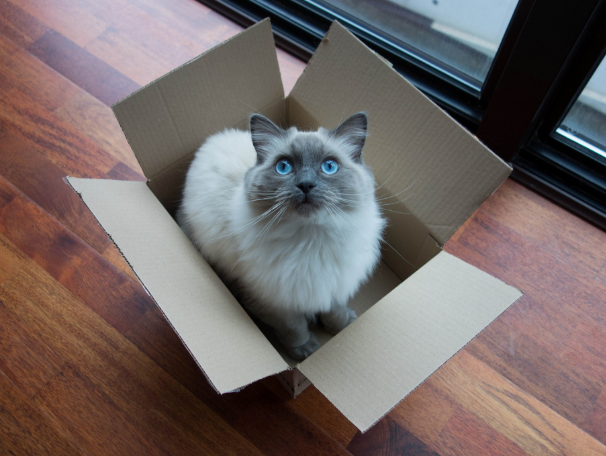
\includegraphics[height=1.5in]{test/boxcat}
	\caption{A boxcat in its natural environment.}
	\label{fig: boxcat}
\end{figure}\vspace{-1em} % will remove 1 white space after image - typically good

\section{Code using Minted}
Code can be added using the \verb|minted| package. The example below is for a Python example, but can be configured other ways. Note that a \verb|--shell-escape| command had to be added to the \TeX Studio build command due to peculiarities with the package. 
Additionally, the \verb|minted| \LaTeX\ package requires python to be installed with the \verb|pygments| package.
This can be done via the '\verb|py -m pip install -U pygments|' console command.

\begin{figure}[!ht]
\begin{minted}[
frame=lines,
framesep=2mm,
baselinestretch=1.2,
bgcolor=gray!13,
fontsize=\footnotesize,
linenos
]{python}
def sumPe(mirror):
    """Returns sum of all electrical power from active machines"""
    sysPe = 0.0

    # for each area
    for area in mirror.Area:
        # reset current sum
        area.cv['Pe'] = 0.0

        # sum each active machine Pe to area agent
        for mach in area.Machines:
            if mach.cv['St'] == 1:
                area.cv['Pe'] += mach.cv['Pe']

        # sum area agent totals to system
        sysPe += area.cv['Pe']

    return sysPe
\end{minted}
	\centering
	\footnotesize
	\caption{Code listing as a figure.}
	\label{fig: codeTest}
\end{figure}\vspace{-1em} % will remove 1 white space after image - typically good

Other packages exist for code insertion, but they may or may not be as pretty. Remember, as with anything, this is totally optional and voluntary...

\pagebreak
\section{Labeled Code Listing}
Sometime you might want to label code as listing - like a person may in \ref{lst: rando code}.
\begin{lstlisting}[caption={Some MATLAB code},label={lst: rando code},language=MATLAB]
for n=1:length(ts)
    
    % Handle basic generation curve
    if ts(n) >= 30 && ts(n) < 90
        % up ramp
        % use first 1/4 cycle of a sin to ramp up
        xs(n) = maxGen*sin( (ts(n)-30) * 2*pi/240); 
    elseif ts(n) >= 150 && ts(n) < 210
        % down ramp
        % use second 1/4 cycle of a sin to ramp down
        xs(n) = maxGen*sin( (ts(n)-150) * 2*pi/240 + pi/2);   
    elseif ts(n) >= 90 && ts(n) < 150
        % held peak
        xs(n) = maxGen;
    else
        % no generation
        xs(n) = 0;
    end
    
    % Handle Cloud cover generation reductions
    if ts(n) >= 45 && ts(n) < 55
        xs(n) = maxGen*.2;
    elseif ts(n) >= 120 && ts(n) < 140
        xs(n) = xs(n)*0.7;
    elseif ts(n) >= 180 && ts(n) < 190
        xs(n) = xs(n)*0.85;
    end
    
end
\end{lstlisting}


\pagebreak
Of course, the listing format may not be very `great', so, a listing environment can precede a minted block to get the best of both yeah?
I mean, if Listing \ref{lst: code 2} is an example then like, yeah.

\begin{lstlisting}[caption={Empty listing before a minted block},label={lst: code 2},language=MATLAB]
\end{lstlisting}\vspace{-2 em}
\begin{minted}[
frame=lines,
framesep=2mm,
baselinestretch=1.2,
bgcolor=gray!13,
fontsize=\footnotesize,
%linenos
]{Matlab}
for n=1:length(ts)
    
    % Handle basic generation curve
    if ts(n) >= 30 && ts(n) < 90
        % up ramp
        % use first 1/4 cycle of a sin to ramp up
        xs(n) = maxGen*sin( (ts(n)-30) * 2*pi/240); 
    elseif ts(n) >= 150 && ts(n) < 210
        % down ramp
        % use second 1/4 cycle of a sin to ramp down
        xs(n) = maxGen*sin( (ts(n)-150) * 2*pi/240 + pi/2);   
    elseif ts(n) >= 90 && ts(n) < 150
        % held peak
        xs(n) = maxGen;
    else
        % no generation
        xs(n) = 0;
    end
    
    % Handle Cloud cover generation reductions
    if ts(n) >= 45 && ts(n) < 55
        xs(n) = maxGen*.2;
    elseif ts(n) >= 120 && ts(n) < 140
        xs(n) = xs(n)*0.7;
    elseif ts(n) >= 180 && ts(n) < 190
        xs(n) = xs(n)*0.85;
    end
    
end
\end{minted}

Right? I mean ideally this should look really good.

 % formatting examples - comment out once a figure, table, equation, and code are included in document

\end{document}